\documentclass{beamer}

\usepackage{textpos}

\setlength{\TPHorizModule}{30mm}
\setlength{\TPVertModule}{\TPHorizModule}
%\textblockorigin{10mm}{10mm} % start everything near the top-left corner

\begin{document}

\begin{frame}
\begin{textblock}{3}(0,0)
This block is 3 modules wide, and is placed with its top left corner
at the `origin' on the page. Note that the length of the block is not
specified in the arguments -- the box will be as long as necessary to
accomodate the text inside it. You need to examine the output of the
text to adjust the positioning of the blocks on the page.
\end{textblock}
\end{frame}

\begin{frame}
\begin{textblock}{2}(2,1)
\textblocklabel{block two}
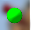
\includegraphics{gravatar.png}
\end{textblock}
\end{frame}

\begin{frame}
\begin{textblock}{3}[0.5,0.5](1,3)
This block is at position (1,3), but because the optional argument
[0.5,0.5] has been given, it is the centre of the block which is
located at that point, rather than the top-left corner.
\end{textblock}
\end{frame}

\end{document}
